\documentclass[tfm,estilo=digital,portada=normativa]{fdi-simplex}

\titulo{Un sistema para ilustrar la plantilla fdi-simplex}
\tituloEN{A system to showcase the fdi-simplex template}

\autor{Meriadoc Brandigamo}
\tutor{Gandalf el Gris}
\cotutor{Elrond Medio-elfo}
\colaboradorExterno{Aragorn hijo de Arathorn (Gondor S.A.)}

% \titulacion recibe solo el nombre del máster, sin el prefijo "Máster
% en": la portada añade "Máster en ..." automáticamente en el TFM.
\titulacion{Ingeniería Informática}
\cursoAcademico{2098/2099}

% --- Campos de la VERSIÓN FINAL (normativa) ---
% \convocatoria y \calificacion solo se rellenan al depositar la versión
% definitiva; aquí van activos para mostrar cómo aparecen en la portada.
\convocatoria{Junio de 2099}
\calificacion{10 (Sobresaliente)}

\palabrasClave{LaTeX, plantilla, TFM, Facultad de Informática}
\keywords{LaTeX, template, master's thesis, Computer Science Faculty}

\addbibresource{bibliografia.bib}

% - OPCIONES DE PERSONALIZACION -

% Usar si se guarda el escudo en otra ubicación
%\logo{img/Escudo_UCM}

% Para cambiar las fuente tipográficas (solo LuaLaTeX/XeLaTeX)
%\setmainfont{Source Serif 4}
%\setmonofont{Source Code Pro}

\begin{document}

\makeportada

\frontmatter

% Normativa (TFM, punto 6): en el TFM el resumen en INGLÉS va primero,
% al contrario que en el TFG. Por eso `abstract' precede a `resumen'.
\begin{abstract}
This document demonstrates the \texttt{fdi-simplex} template for
writing the report of a Master's Thesis at the Faculty of
Computer Science of the Complutense University of Madrid. The
template provides a normalized cover page, bilingual abstract and
keyword environments, and biblatex integration. For a Master's
thesis the regulations ask for an English abstract of roughly half
a page, placed before the Spanish one.
\keywords{LaTeX, template, master's thesis, Computer Science Faculty, Complutense University of Madrid}
\end{abstract}

\begin{resumen}
Este documento demuestra el uso de la plantilla \texttt{fdi-simplex}
para redactar la memoria de un Trabajo de Fin de Máster en la
Facultad de Informática de la Universidad Complutense de Madrid. La
plantilla incluye la portada normalizada, entornos bilingües para
resumen y palabras clave, e integración con biblatex.
\palabrasClave{LaTeX, plantilla, TFM, Facultad de Informática, Universidad Complutense de Madrid}
\end{resumen}

\tableofcontents

\mainmatter

\chapter{Introducción}

Este capítulo introduce los antecedentes, objetivos y plan de
trabajo de la memoria, tal y como exige la normativa del Trabajo
de Fin de Máster de la Facultad de Informática
(\href{https://informatica.ucm.es/normativa-tfm-2425}{informatica.ucm.es/normativa-tfm-2425}).

\section{Normativa}

\begin{itemize}\setlength{\itemsep}{0pt}
  \item Extensión mínima: 50 páginas.
  \item Máximo 10 palabras clave en cada idioma.
  \item El resumen en inglés debe ocupar aproximadamente media
        página y precede al resumen en castellano.
  \item Todo material no original (texto, figuras, código) debe
        citarse y respetar licencias.
  \item El estudiante debe firmar y adjuntar la \emph{declaración
        responsable sobre autoría y uso ético de herramientas de
        inteligencia artificial}.
\end{itemize}

\section{Antecedentes}

La Facultad de Informática de la UCM ha utilizado durante más de
una década el sistema TeXiS~\cite{texis} para sus memorias de
tesis y trabajos de fin de carrera. Esta cáscara ayuda a preparar
documentos complejos con buenas prácticas, pero al ser una
cáscara y no una plantilla, es más complicada de integrar con
otros sistemas, además de no incentivar el aprendizaje de LaTeX
por los usuarios.

\section{Objetivos}

Los objetivos de este trabajo son:
\begin{itemize}
  \item Disponer de una plantilla moderna basada en LuaLaTeX.
  \item Separar los aspectos normativos de los estéticos.
  \item Ofrecer una base mínima que no interfiera con los
        paquetes que cada estudiante decida usar.
\end{itemize}

\chapter{Desarrollo}

El cuerpo principal de la memoria describe el trabajo realizado.
En este ejemplo, demostramos algunas construcciones típicas: una
cita bibliográfica~\parencite{knuth1986} y referencias cruzadas a
la sección~\ref{sec:arquitectura}. La cita anterior es parentética
(autor y año dentro del paréntesis); cuando el autor ya forma parte
de la frase conviene usar \verb|\textcite|, que sólo encierra el
año: \textcite{tolkien1954lord} cuenta cómo Bilbo decía a menudo
que solo había un camino y que era como un río caudaloso; nacía
en el umbral de todas las puertas, y todos los senderos eran ríos
tributarios. "Es muy peligroso, Frodo, cruzar la puerta", solía
decirme. "Vas hacia el Camino, y si no cuidas tus pasos no sabes
hacia donde te arrastrarán".

Las imágenes se guardan en la carpeta \texttt{img/} y se incluyen con
\verb|\includegraphics| dentro de un entorno \texttt{figure}, que les
añade un pie y una etiqueta para poder referenciarlas, como en la
figura~\ref{fig:bolson-cerrado}. Conviene dar el ancho en relación con
\verb|\textwidth| y se puede omitir la extensión del archivo. Si la
imagen no es propia, el pie debe indicar su autoría y procedencia.

\begin{figure}
  \centering
  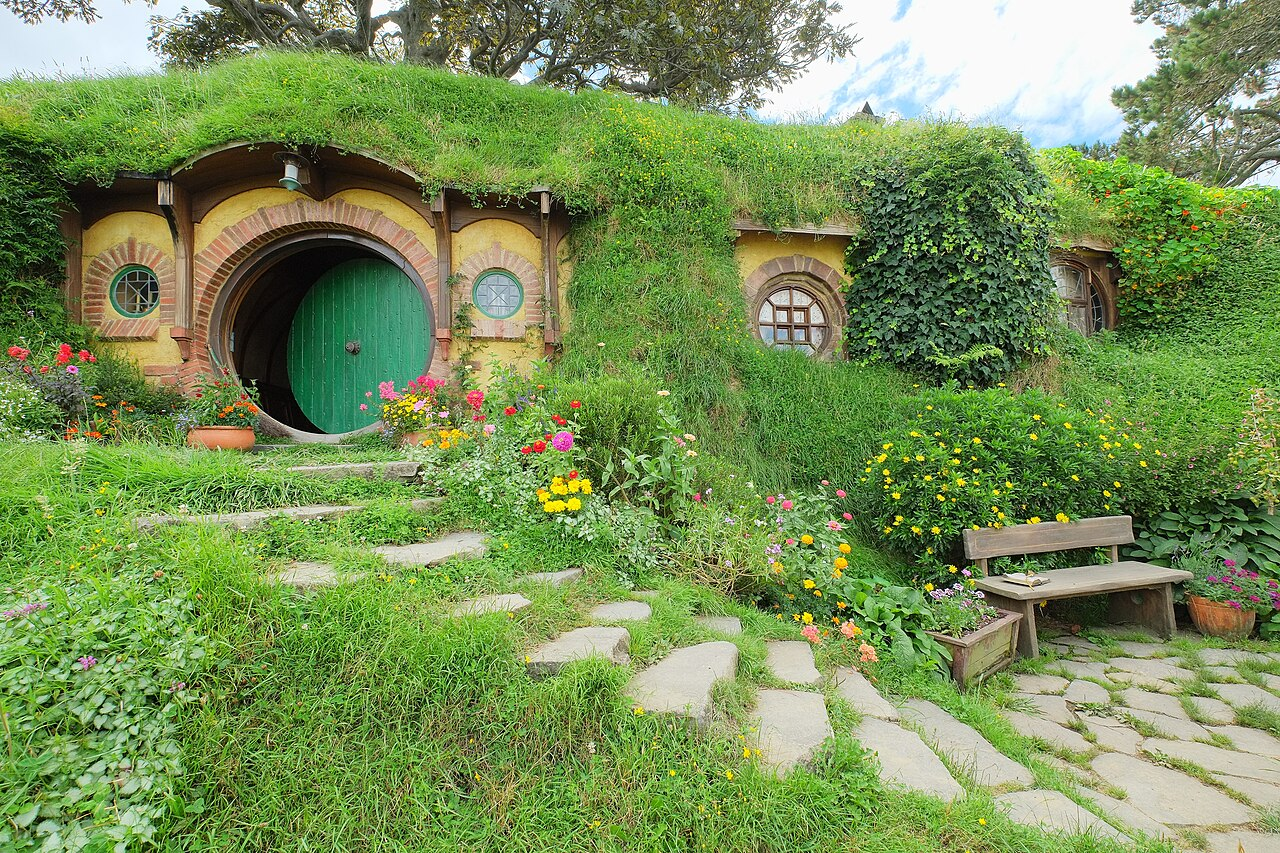
\includegraphics[width=0.8\textwidth]{img/bolson_cerrado}
  % El argumento opcional es la versión corta para el índice de figuras.
  \caption[Bolsón Cerrado]{Bolsón Cerrado, residencia de los Bolsón, en
    el decorado de Hobbiton (Matamata, Nueva Zelanda). Fotografía de
    Pseudopanax (2018), en dominio público. Fuente: Wikimedia Commons,
    \url{https://commons.wikimedia.org/wiki/File:Baggins_residence_'Bag_End'.jpg}.}
  \label{fig:bolson-cerrado}
\end{figure}

\section{Arquitectura}
\label{sec:arquitectura}

La arquitectura del sistema sigue el patrón de separación entre
normativa y estilo. La clase \texttt{fdi-simplex} implementa los
requisitos obligatorios de la normativa UCM-FDI; el aspecto
visual concreto queda delegado a la opción \texttt{estilo}, como
resume la tabla~\ref{tab:estilos}. Las tablas se componen con el entorno
\texttt{tabular} dentro de un \texttt{table} que, igual que
\texttt{figure}, es un flotante: \LaTeX{} decide dónde colocarlo, y
no siempre queda junto al texto que lo menciona.

\begin{table}
  \centering
  \begin{tabular}{|l|l|}
    \hline
    \textbf{Estilo} & \textbf{Descripción} \\
    \hline
    \texttt{digital} & Lora, enlaces en color, pensado para leer en pantalla \\
    \hline
    \texttt{clasico} & Reminiscente de TeXiS, a dos caras \\
    \hline
    \texttt{minimo} & Casi sin personalizar, para partir de él \\
    \hline
  \end{tabular}
  \caption{Estilos disponibles en la clase.}
  \label{tab:estilos}
\end{table}

\section{Implementación}

La implementación se basa en la clase KOMA-Script
\texttt{scrbook} \autocite{kohm2004koma}, con soporte nativo para UTF-8 mediante
LuaLaTeX.

\chapter{Conclusiones}

Se ha implementado una plantilla moderna para los trabajos de
fin de estudios de la Facultad de Informática, compatible con
LuaLaTeX y con una separación clara entre los aspectos
normativos y los estéticos.

\chapter{Conclusions}

A modern template for the final-year projects of the Faculty of
Computer Science has been implemented, compatible with Lua\LaTeX{}
and with a clear separation between regulatory and aesthetic concerns.


\backmatter

% A diferencia del TFG, el TFM es individual: no lleva el entorno
% `contribucion' (reservado a los trabajos en grupo).

\printbibliography[heading=bibintoc]

\end{document}
